\section{Paketstruktur}
Dieser Abschnitt beschreibt die strukturelle Gliederung des Projektes in einem Paketdiagramm, dargestellt in Abbildung \ref{Paketstruktur}.

Die Pakete \textit{RobotSoftware} und \textit{Server} werden getrennt betrachtet, da es eine physikalische Trennung zwischen den Geräten gibt, auf denen die jeweiligen Pakete vorhanden sein müssen.

Im \textit{Common}-Paket sind alle Klassen enthalten, die sowohl vom \textit{Robot}- als auch vom \textit{Server}-Paket genutzt werden. 
So sind die Datentypen \textit{Position} und \textit{Task} enthalten. 
Eine Möglichkeit zur Unterscheidung von \textit{Tasks} ist wichtig, da zwischen vom \textit{Server} zugeteilten \textit{Tasks}, insbesondere Taxi- und Krankenhaustransporten, und vom \textit{Robot} selbst zugeteilten Ladestationen als Ziel unterschieden werden muss. 

Das Paket \textit{Robot} enthält das Paket \textit{HardwareInterfaces}, welches die Möglichkeiten schafft, die Hardwareschnittstellen des \textit{Robots} direkt anzusprechen. 
Das Paket \textit{RobotControl} enthält Klassen zur Steuerung und Speicherung des Zustandes des \textit{Robots}, sowie die \emph{Handler}, die den Hardwareschnittstellen übergeben werden.

Der Server hat Klassen zur Verwaltung der \textit{Robots} und ihren zugehörigen \textit{Tasks}. 
Außerdem sind im \textit{Server} Paket auch Klassen zur Kommunikation mit dem \textit{Hospital} und den Taxikunden vorhanden.

\begin{figure}[H]
\centering
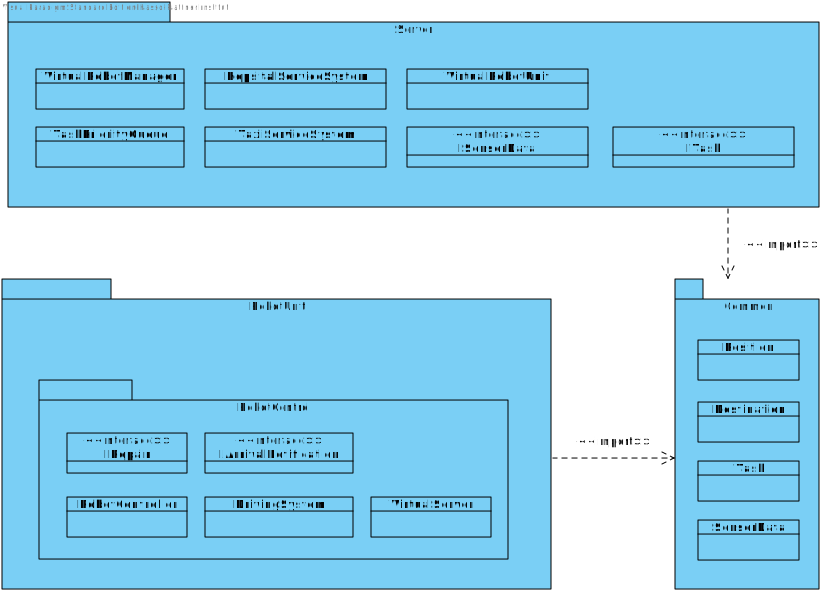
\includegraphics[height=0.8\textwidth, angle=90]{img/6_paketdiagramm}
\caption{Paketdiagramm zur strukturellen Gliederung der Software}
\label{Paketstruktur}
\end{figure}
